%%%%%%%%%%%%%%%%%%%%%%%%%%%%%%%%%%%%%%%%%
% "ModernCV" CV and Cover Letter
% LaTeX Template
% Version 1.1 (9/12/12)
%
% This template has been downloaded from:
% http://www.LaTeXTemplates.com
%
% Original author:
% Xavier Danaux (xdanaux@gmail.com)
%
% License:
% CC BY-NC-SA 3.0 (http://creativecommons.org/licenses/by-nc-sa/3.0/)
%
% Important note:
% This template requires the moderncv.cls and .sty files to be in the same 
% directory as this .tex file. These files provide the resume style and themes 
% used for structuring the document.
%
%%%%%%%%%%%%%%%%%%%%%%%%%%%%%%%%%%%%%%%%%

%----------------------------------------------------------------------------------------
%	PACKAGES AND OTHER DOCUMENT CONFIGURATIONS
%----------------------------------------------------------------------------------------

\documentclass[10pt,a4paper,sans]{moderncv} % Font sizes: 10, 11, or 12; paper sizes: a4paper, letterpaper, a5paper, legalpaper, executivepaper or landscape; font families: sans or roman
\usepackage[utf8]{inputenc}
\usepackage[export]{adjustbox}

%\usepackage[francais]{babel}
\moderncvstyle{casual} % CV theme - options include: 'casual' (default), 'classic', 'oldstyle' and 'banking'
\moderncvcolor{purple} % CV color - options include: 'blue' (default), 'orange', 'green', 'red', 'purple', 'grey' and 'black'
%\usepackage{lipsum} % Used for inserting dummy 'Lorem ipsum' text into the template

\usepackage[scale=0.85]{geometry} % Reduce document margins %0.75
%\setlength{\hintscolumnwidth}{3cm} % Uncomment to change the width of the dates column
%\setlength{\makecvtitlenamewidth}{10cm} % For the 'classic' style, uncomment to adjust the width of the space allocated to your name

\hyphenation{}
%----------------------------------------------------------------------------------------
%	NAME AND CONTACT INFORMATION SECTION
%----------------------------------------------------------------------------------------

\firstname{Julien} % Your first name
\familyname{Aldon} % Your last name

%----------------------------------------------------------------------------------------

\begin{document}
% \hspace*{-1.5cm}
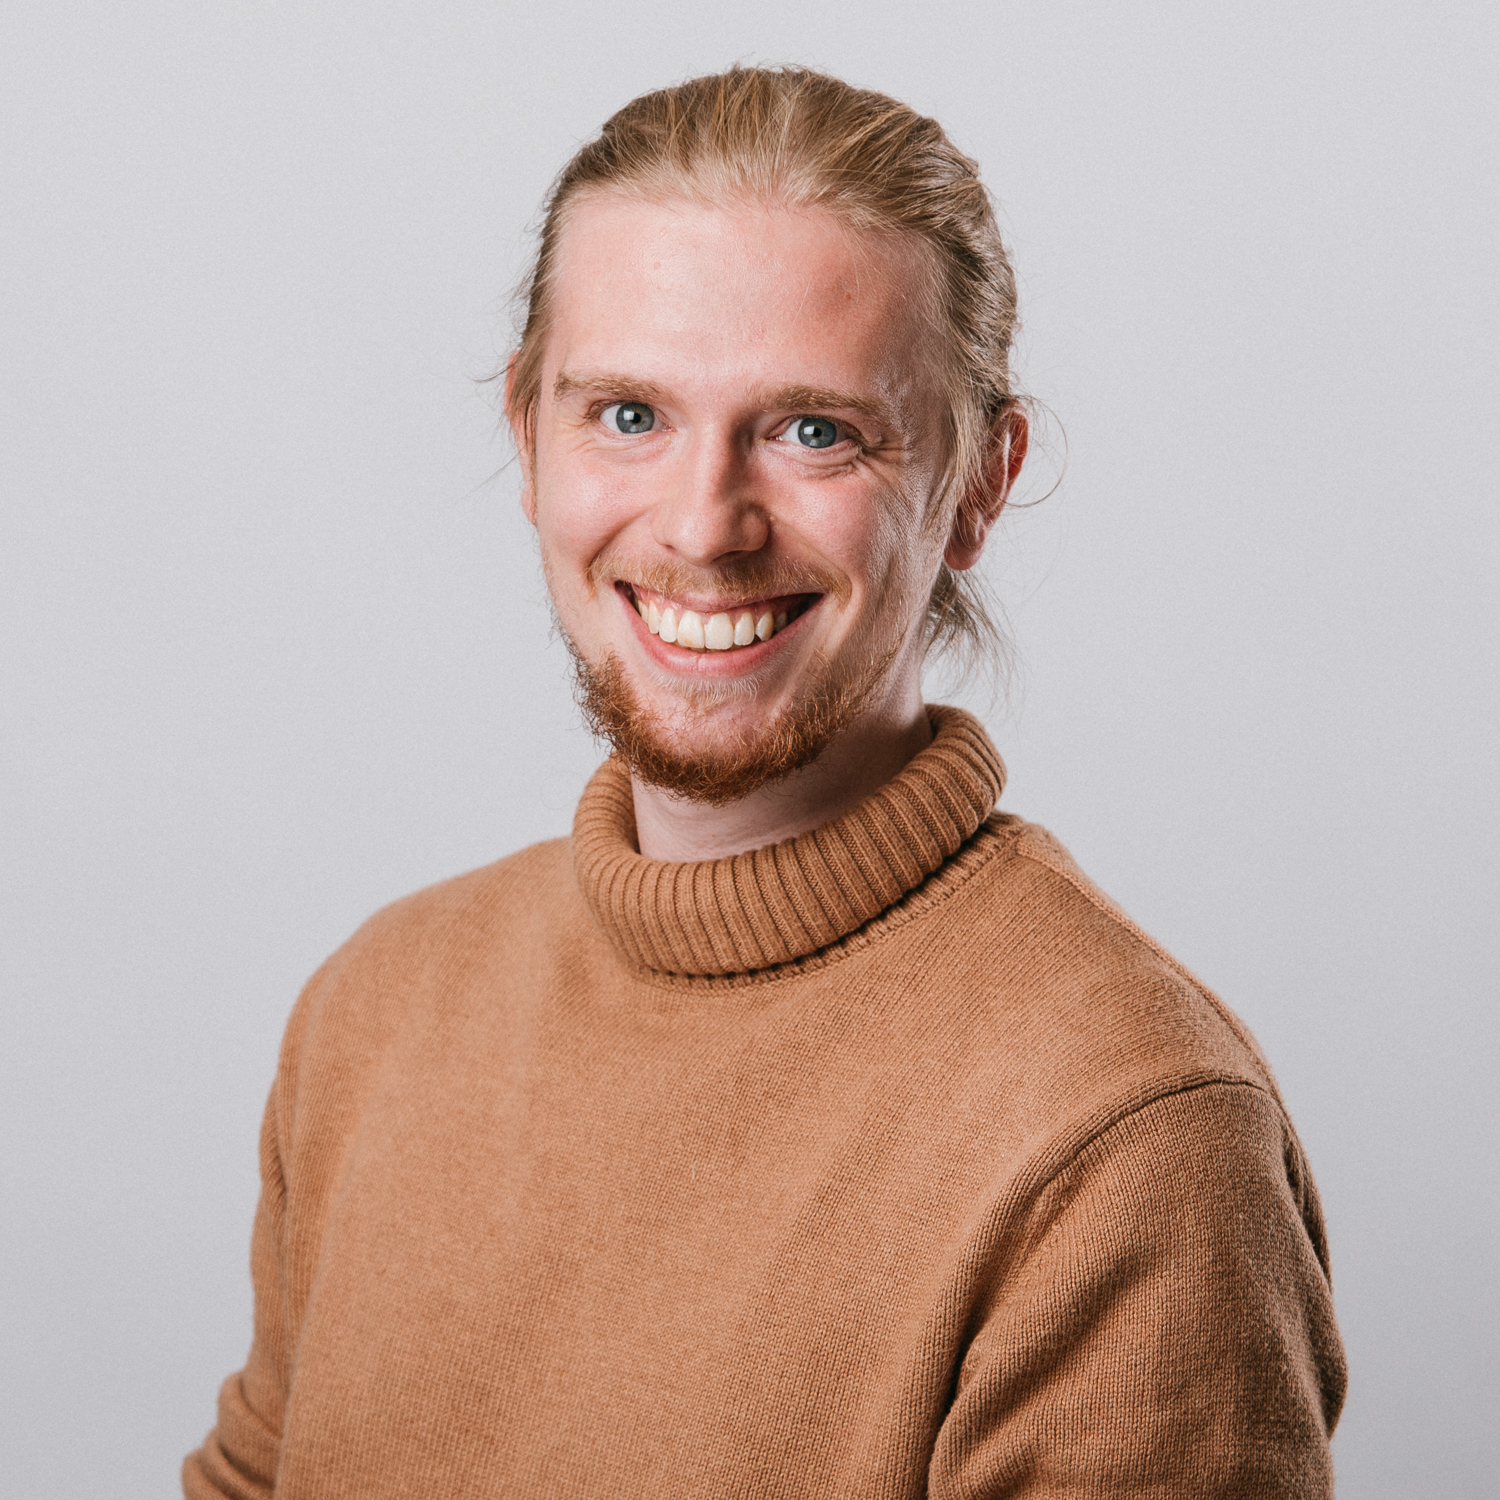
\includegraphics[height=70pt]{pictures/julien.jpg}
\hspace{12.8cm}

\includegraphics[height=70pt]{pictures/qrcode_portfolio.png}

\makecvtitle % Print the CV title

\vspace*{-1.5cm}
\begin{flushright}
né le 6 octobre 1998 à Lyon, France\\
courriel : julien.aldon@wanadoo.fr\\

\end{flushright} %\\[-10cm]
% \begin{center} Réponse à l'appel d'offre : "Aide à la conception et à la génération d'activités d'apprentissage ludiques adaptables".
% \begin{center}Cherche un emploi dans les domaines du développement, de la programmation, du jeu vidéo ou de la pédagogie\end{center}
% \begin{center}Responsable Pédagogique Epitech\end{center}
\begin{center}En recherche d'un CDI en développement Pyhton\end{center}
%----------------------------------------------------------------------------------------
%	EDUCATION SECTION
%----------------------------------------------------------------------------------------
\vspace*{-0.2cm}
\section{Situation actuelle}
\cventry{}{Developpeur Fullstack au sein de l'équipe de developpement d'Epitech}{2024}{}{}{}
 %Au pair

%----------------------------------------------------------------------------------------
%	WORK EXPERIENCE SECTION
%----------------------------------------------------------------------------------------

\section{Expérience professionnelle}
\cventry{Juillet 2017 – Dec. 2017}{Stage à Adecco IT Services}{Capacity management}{Python}{}{}
\cventry{Sept. 2018 – Mars 2019}{Stage en alternance à la Code Academy}{Assistant pédagogique}{}{}{}
\cventry{Mars. 2019 - Aout 2020}{Stage à Wecandoo}{Fullstack web}{I18n et transition vers React}{}{}
\cventry{Oct. 2020 - Mars 2021}{Stage à Stackeo}{Fullstack web}{Package manager en Python, Django}{}{}
\cventry{Mars 2021 - Aout 2021}{Stage à Grame CNCM}{Recherche \& developpement INScore}{}{}{}
\cventry{Aout 2021 - Fevrier 2024}{Responsable pédagogique Epitech MSC}{Pédagogie}{Spécialité Web et Python}{}{}
\cventry{Fevrier 2024 - Octobre 2025}{Développement des outils de la pédagogie à Epitech}{Fullstack}{Typescript, React, Next, Nest, Express}{}{}

%----------------------------------------------------------------------------------------
%	COMPUTER SKILLS SECTION
%----------------------------------------------------------------------------------------
\vspace*{-0.2cm}
\section{Programmation}

\cvitem{Langages maîtrisés}{C, C++, C\# (Unity), Python, JavaScript, Typescript et Technologies associées (React, VueJS \dots), HTML5, CSS, \LaTeX, Php, Ruby, SQL (PgSQL, mariadb), INScore, GdScript (Godot)}
\cvitem{Languages en apprentissage}{Rust}


\vspace*{-0.2cm}
\section{Projets}
\cventry{}{Tous mes projets sont diponibles dans mon port-folio}{}{\href{https://julienaldon.github.io/Port-Folio/}{Ici}}{Ou en Scanant le QRcode ci dessus}{}{}
% \cventry{2019-2020}{Escape the volcano}{Personel}{Jeu vidéo réalisé après l'avoir réalisé durant un cours de design de jeu en Russie}{\href{https://github.com/JulienAldon/EscapeTheVolcano}{Disponible ici}}{}{}
\cventry{2018-2020}{JAMMEE}{Epitech}{Projet de fin d'études, il s'agit d'un logiciel de musique assistée par ordinateur dans un navigateur}{\href{https://jammee.io/}{Disponible ici}}{}{}
\cventry{2018}{Publify}{Epitech}{Projet utilisant l'api Spotify permettant de synchroniser des playlists}{\href{https://github.com/JulienAldon/Publify}{Disponible ici}}{}{}
% \cventry{2017}{Raytracer2}{Epitech}{Projet réalisé lors de ma première année à Epitech, ce projet a été réalisé en groupe}{\href{https://github.com/JulienAldon/Epitech\_Raytracer2}{Disponible ici}}{}{}

\vspace*{-0.2cm}
\section{Formation}
\cventry{2021}{Diplomé Master 2}{Epitech}{Lyon}{}{}
\cventry{2019-2020}{Année en Russie}{à l'université d'état de télécommunication}{St-Peterbourg}{}{}
\cventry{2019}{Bachelor}{Epitech}{Lyon}{}{}{}
% \cventry{2016}{Baccalauréat Scientifique S-SI, mention AB}{Lycée Brossolette, Villeurbanne} {}{}{}  % 

% \cventry{2013 – 2016}{Seconde générale puis première S et terminale S, option SI, spécialité Informatique et Sciences du Numérique (ISN), option latin de la cinquième à la terminale} 
% {}{}{}{} % 

% \cventry{Sept. 2009 – Juin 2013}{Collège Fénelon, Lyon 6eme} 
% {Classe européenne}{}{}{} % Arguments not required can be left empty

%----------------------------------------------------------------------------------------
%	LANGUAGES SECTION
%----------------------------------------------------------------------------------------
\vspace*{-0.2cm}
\section{Langues}

\cvitemwithcomment{Français}{Langue maternelle}{}
\cvitemwithcomment{Anglais}{Niveau C1}{Maîtrise de l'écrit et de l'oral, De juin à août 2016 je suis parti aux États Unis, en Pennsylvanie.}
% \cvitemwithcomment{Allemand}{Niveau B1}{J'ai participé à plusieurs échanges scolaires avec l'Allemagne~: séjours à Hanovre et Berlin.}
% \cvitemwithcomment{Russe}{Débutant}{Dans le cadre de mon année à l'étranger j'ai appris quelques rudiments de Russe.}
% \cvitemwithcomment{Voyages}{}{J'ai organisé et effectué de nombreux voyages en Europe avec des groupes.}

%Main Fields
 
%----------------------------------------------------------------------------------------
%	INTERESTS SECTION
%----------------------------------------------------------------------------------------
% \vspace*{-0.2cm}
% \section{Centres d'intérêt}
%  
%\renewcommand{\listitemsymbol}{-~} % Changes the symbol used for lists
%  \cventry{2016}{Baccalauréat Scientifique S-SI, mention AB}{Lycée Brossolette, Villeurbanne} {}{}{}
% \cventry{Musique}{J'ai fait sept années de violon au sein de l'École Nationale de Musique de Villeurbanne}{}{}{}{}
% \cventry{}{Pendant cette période j'ai fait partie de l'orchestre de la promotion}{2nd violon}{}{}{}
% \cventry{Sports}{Tennis : dans le club Rhône Sportif à Villeurbanne}{}{}{}{}
% \cventry{}{Natation : 8 années au club ALAP à Villeurbanne}{compétitions régulières avec l'équipe du club}{}{}{}
% \cventry{Dessin}{J'ai suivi pendant les trois années de lycée, l'option arts plastiques}{j'ai participé au projet de décoration de l'établissement avec des \oe uvres intégrées dans son architecture}{}{}{}
% \cventry{}{Dans l'École de dessin de Villeurbanne, \textit{L'Atelier}, j'ai contribué à l'exposition de l'école par mes \oe uvres\textit{}}{}{}{}{}
% % 
%----------------------------------------------------------------------------------------
%	COVER LETTER
%----------------------------------------------------------------------------------------

% To remove the cover letter, comment out this entire block
% 
% \clearpage
% 
% \recipient{HR Departmnet}{Corporation\\123 Pleasant Lane\\12345 City, State} % Letter recipient
% \date{\today} % Letter date
% \opening{Dear Sir or Madam,} % Opening greeting
% \closing{Sincerely yours,} % Closing phrase
% \enclosure[Attached]{curriculum vit\ae{}} % List of enclosed documents
% 
% \makelettertitle % Print letter title
% 
% \lipsum[1-3] % Dummy text
% 
% \makeletterclosing % Print letter signature

%----------------------------------------------------------------------------------------

\end{document}
